\section{Дополнение к основным результатам}

\subsection{Визуализация абляционных исследований}

% \enlargethispage{2\baselineskip}

Для оценки предсказаний различных моделей приводится визуализация результатов 
прогнозирования на тестовой выборке набора данных ETTh1 в рамках абляционных исследований, 
что позволяет провести качественное сравнение.

% Ablation 1
% 5 plots (for horizons: {24, 48, 168, 336, 720}) model A
% 5 plots (for horizons: {24, 48, 168, 336, 720}) model B

\begin{table}[H]
    \centering
    \caption{Примеры прогнозирования из набора данных ETTh1 в ходе абляционных исследований 
    \textit{ConvStem вместо TokenEmbedding} (см. раздел~\ref{sec:ablations1}) в настройках 
    \texttt{input-96-predict-horizon}. {\color{blue} Синие} линии - истинные значения, 
    {\color{orange} оранжевые} линии - предсказания модели, {\color{green} зеленые} - входные данные 
    длиной 96. }
    \vspace{5pt}
    \label{tab:ablations1}
    \resizebox{0.98\textwidth}{!}{
    \setlength{\tabcolsep}{4pt}        % adjust horizontal padding
    \renewcommand{\arraystretch}{1.5}  % big body‐row spacing
    \begin{tabular}{lccccc}
      \toprule
      % first header row, pulled in by negative space
      \multirow{2}{*}{\rotatebox{90}{{} Model}} \\[-2.25em]
        & \multicolumn{5}{c}{{Horizon}} \\[-0.25em]
      \cmidrule(lr){2-6} \\[-2.25em]
      % second header row, also pulled in
        & {24}
        & {48}
        & {168}
        & {336}
        & {720} \\[-0.15em]
      \midrule
  
      % body rows with the large 1.5× spacing

      \rotatebox{90}{{} Informer}
        & \includegraphics[width=2.9cm]{Ablation 1/24A.pdf}
        & \includegraphics[width=2.9cm]{Ablation 1/48A.pdf}
        & \includegraphics[width=2.9cm]{Ablation 1/168A.pdf}
        & \includegraphics[width=2.9cm]{Ablation 1/336A.pdf}
        & \includegraphics[width=2.9cm]{Ablation 1/720A.pdf} \\[1.4em]
  
      \rotatebox{90}{{} {} {} ConvStem}
        & \includegraphics[width=2.9cm]{Ablation 1/24B.pdf}
        & \includegraphics[width=2.9cm]{Ablation 1/48B.pdf}
        & \includegraphics[width=2.9cm]{Ablation 1/168B.pdf}
        & \includegraphics[width=2.9cm]{Ablation 1/336B.pdf}
        & \includegraphics[width=2.9cm]{Ablation 1/720B.pdf} \\[1.4em]
    \end{tabular}
    }
\end{table}
% \vspace{-40pt}

% Ablation 2
% 5 plots (for horizons: {24, 48, 168, 336, 720}) model A
% 5 plots (for horizons: {24, 48, 168, 336, 720}) model B

\begin{table}[H]
    \centering
    \caption{Примеры прогнозирования из набора данных ETTh1 в ходе абляционных исследований 
    \textit{ProbSparse $\to$ FAVOR+} (см. раздел~\ref{sec:ablations2}) в настройках 
    \texttt{input-96-predict-horizon}.}
    \vspace{5pt}
    \label{tab:ablations2}
    \resizebox{0.98\textwidth}{!}{
    \setlength{\tabcolsep}{4pt}        % adjust horizontal padding
    \renewcommand{\arraystretch}{1.5}  % big body‐row spacing
    \begin{tabular}{lccccc}
      \toprule
      % first header row, pulled in by negative space
      \multirow{2}{*}{\rotatebox{90}{{} Model}} \\[-2.25em]
        & \multicolumn{5}{c}{{Horizon}} \\[-0.25em]
      \cmidrule(lr){2-6} \\[-2.25em]
      % second header row, also pulled in
        & {24}
        & {48}
        & {168}
        & {336}
        & {720} \\[-0.15em]
      \midrule
  
      % body rows with the large 1.5× spacing

      \rotatebox{90}{{} Informer}
        & \includegraphics[width=2.9cm]{Ablation 2/24A.pdf}
        & \includegraphics[width=2.9cm]{Ablation 2/48A.pdf}
        & \includegraphics[width=2.9cm]{Ablation 2/168A.pdf}
        & \includegraphics[width=2.9cm]{Ablation 2/336A.pdf}
        & \includegraphics[width=2.9cm]{Ablation 2/720A.pdf} \\[1.4em]
  
      \rotatebox{90}{{} {} {} w/ FAVOR+}
        & \includegraphics[width=2.9cm]{Ablation 2/24B.pdf}
        & \includegraphics[width=2.9cm]{Ablation 2/48B.pdf}
        & \includegraphics[width=2.9cm]{Ablation 2/168B.pdf}
        & \includegraphics[width=2.9cm]{Ablation 2/336B.pdf}
        & \includegraphics[width=2.9cm]{Ablation 2/720B.pdf} \\[1.4em]
    \end{tabular}
    }
\end{table}
% \vspace{-40pt}
\vfill\newpage

% Ablation 3
% 5 plots (for horizons: {24, 48, 168, 336, 720}) model A
% 5 plots (for horizons: {24, 48, 168, 336, 720}) model B

\begin{table}[H]
    \centering
    \caption{Примеры прогнозирования из набора данных ETTh1 в ходе абляционных исследований 
    \textit{Informer с модулем декомпозиции} (см. раздел~\ref{sec:ablations3}) в настройках 
    \texttt{input-96-predict-horizon}.}
    \vspace{5pt}
    \label{tab:ablations3}
    \resizebox{0.98\textwidth}{!}{
    \setlength{\tabcolsep}{4pt}        % adjust horizontal padding
    \renewcommand{\arraystretch}{1.5}  % big body‐row spacing
    \begin{tabular}{lccccc}
      \toprule
      % first header row, pulled in by negative space
      \multirow{2}{*}{\rotatebox{90}{{} Model}} \\[-2.25em]
        & \multicolumn{5}{c}{{Horizon}} \\[-0.25em]
      \cmidrule(lr){2-6} \\[-2.25em]
      % second header row, also pulled in
        & {24}
        & {48}
        & {168}
        & {336}
        & {720} \\[-0.15em]
      \midrule
  
      % body rows with the large 1.5× spacing

      \rotatebox{90}{{} Informer}
        & \includegraphics[width=2.9cm]{Ablation 3/24A.pdf}
        & \includegraphics[width=2.9cm]{Ablation 3/48A.pdf}
        & \includegraphics[width=2.9cm]{Ablation 3/168A.pdf}
        & \includegraphics[width=2.9cm]{Ablation 3/336A.pdf}
        & \includegraphics[width=2.9cm]{Ablation 3/720A.pdf} \\[1.4em]
  
      \rotatebox{90}{{} {} {} w/ s.decomp}
        & \includegraphics[width=2.9cm]{Ablation 3/24B.pdf}
        & \includegraphics[width=2.9cm]{Ablation 3/48B.pdf}
        & \includegraphics[width=2.9cm]{Ablation 3/168B.pdf}
        & \includegraphics[width=2.9cm]{Ablation 3/336B.pdf}
        & \includegraphics[width=2.9cm]{Ablation 3/720B.pdf} \\[1.4em]
    \end{tabular}
    }
\end{table}

\subsection{Визуализация основных результатов}

% Main
% 4 plots (for horizons: 336) Convformer, Informer, Performer, Autoformer

\begin{figure}[h!]
    \centering
    % First image
    \begin{subfigure}[b]{0.24\textwidth}
        \centering
        \includegraphics[width=\textwidth]{main/336A.pdf}
        \caption{Convformer}
        \label{fig:img1}
    \end{subfigure}
    % Second image
    \begin{subfigure}[b]{0.24\textwidth}
        \centering
        \includegraphics[width=\textwidth]{main/336B.pdf}
        \caption{Informer}
        \label{fig:img2}
    \end{subfigure}
    % Third image
    \begin{subfigure}[b]{0.24\textwidth}
        \centering
        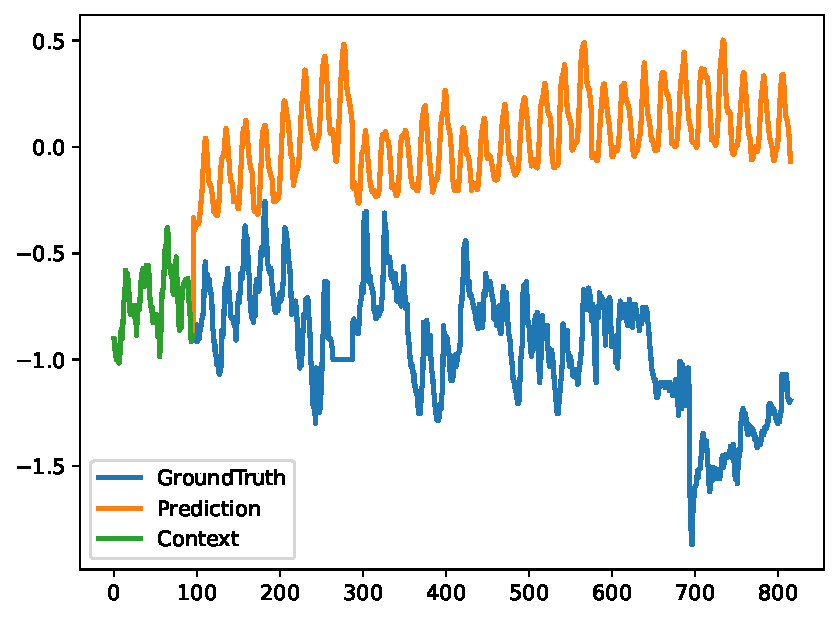
\includegraphics[width=\textwidth]{main/336C.pdf}
        \caption{Performer}
        \label{fig:img3}
    \end{subfigure}
    % Fourth image
    \begin{subfigure}[b]{0.24\textwidth}
        \centering
        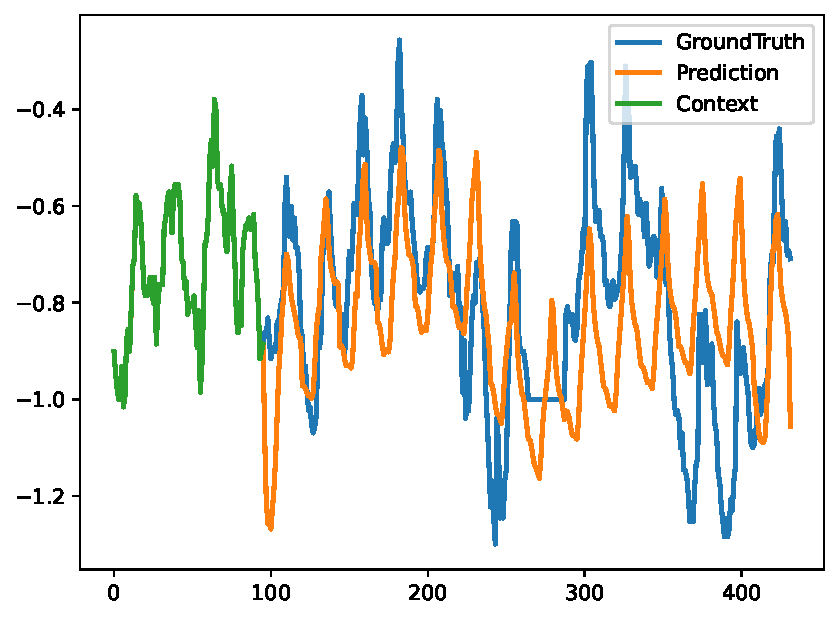
\includegraphics[width=\textwidth]{main/336D.pdf}
        \caption{Autoformer}
        \label{fig:img4}
    \end{subfigure}
    
    \caption{Примеры прогнозирования из набора данных ETTh1 в настройках 
    \texttt{input-96-predict-336}.}
    \label{fig:four_images}
\end{figure}

% \enlargethispage{2\baselineskip}
% \begin{table}[H]
%     \centering
%     \caption{Примеры прогнозирования из набора данных ETTh1 в настройках 
%     \texttt{input-96-predict-horizon}. {\color{blue} Синие} линии — истинные значения, 
%     {\color{orange} оранжевые} линии — предсказания модели. Первая часть длиной 96 
%     является входными данными.}
%     \label{tab:models-horizons}
%     \resizebox{0.98\textwidth}{!}{
%     \setlength{\tabcolsep}{4pt}        % adjust horizontal padding
%     \renewcommand{\arraystretch}{1.5}  % big body‐row spacing
%     \begin{tabular}{lccccc}
%       \toprule
%       % first header row, pulled in by negative space
%       \multirow{2}{*}{\rotatebox{90}{{} Model}} \\[-3.25em]
%         & \multicolumn{5}{c}{{Horizon}} \\[-0.25em]
%       \cmidrule(lr){2-6} \\[-3.25em]
%       % second header row, also pulled in
%         & {24}
%         & {48}
%         & {168}
%         & {336}
%         & {720} \\[-0.25em]
%       \midrule
  
%       % body rows with the large 1.5× spacing
%       \rotatebox{90}{Convformer}
%         & \includegraphics[width=2.9cm]{24_Convformer.pdf}
%         & \includegraphics[width=2.9cm]{48_Convformer.pdf}
%         & \includegraphics[width=2.9cm]{168_Convformer.pdf}
%         & \includegraphics[width=2.9cm]{336_Convformer.pdf}
%         & \includegraphics[width=2.9cm]{720_Convformer.pdf} \\[1.4em]
  
%       \rotatebox{90}{{} Informer}
%         & \includegraphics[width=2.9cm]{24_Informer.pdf}
%         & \includegraphics[width=2.9cm]{48_Informer.pdf}
%         & \includegraphics[width=2.9cm]{168_Informer.pdf}
%         & \includegraphics[width=2.9cm]{336_Informer.pdf}
%         & \includegraphics[width=2.9cm]{720_Informer.pdf} \\[1.4em]
  
%       \rotatebox{90}{Autoformer}
%         & \includegraphics[width=2.9cm]{24_Autoformer.pdf}
%         & \includegraphics[width=2.9cm]{48_Autoformer.pdf}
%         & \includegraphics[width=2.9cm]{168_Autoformer.pdf}
%         & \includegraphics[width=2.9cm]{336_Autoformer.pdf}
%         & \includegraphics[width=2.9cm]{720_Autoformer.pdf} \\[1.4em]
  
%       \rotatebox{90}{{} Reformer}
%         & \includegraphics[width=2.9cm]{24_Reformer.pdf}
%         & \includegraphics[width=2.9cm]{48_Reformer.pdf}
%         & \includegraphics[width=2.9cm]{168_Reformer.pdf}
%         & \includegraphics[width=2.9cm]{336_Reformer.pdf}
%         & \includegraphics[width=2.9cm]{720_Reformer.pdf} \\[1.4em]
  
%       \rotatebox{90}{ConvStem}
%         & \includegraphics[width=2.9cm]{24_ConvStem.pdf}
%         & \includegraphics[width=2.9cm]{48_ConvStem.pdf}
%         & \includegraphics[width=2.9cm]{168_ConvStem.pdf}
%         & \includegraphics[width=2.9cm]{336_ConvStem.pdf}
%         & \includegraphics[width=2.9cm]{720_ConvStem.pdf} \\[1.4em]
  
%       \rotatebox{90}{{} {} Decomp}
%         & \includegraphics[width=2.9cm]{24_Decomp.pdf}
%         & \includegraphics[width=2.9cm]{48_Decomp.pdf}
%         & \includegraphics[width=2.9cm]{168_Decomp.pdf}
%         & \includegraphics[width=2.9cm]{336_Decomp.pdf}
%         & \includegraphics[width=2.9cm]{720_Decomp.pdf} \\[1.4em]
  
%       \rotatebox{90}{{} {} {} FAVOR}
%         & \includegraphics[width=2.9cm]{24_FAVOR.pdf}
%         & \includegraphics[width=2.9cm]{48_FAVOR.pdf}
%         & \includegraphics[width=2.9cm]{168_FAVOR.pdf}
%         & \includegraphics[width=2.9cm]{336_FAVOR.pdf}
%         & \includegraphics[width=2.9cm]{720_FAVOR.pdf} \\[1.4em]
%     \end{tabular}
%     }
% \end{table}
